%%%%%%%%%%%%%%%%%%%%%%%%%%%%%%%%%%%%%%%%%%%%%%%%%%%%%%%%%%%%%%%%
%                                                              %
%                                                              %
% Macallyster S. Edmondson                                     %
%                                                              %
% ECE351-53                                                    %
%                                                              %
% Lab #4                                                       %
%                                                              %
% 02/15/2022                                                   %
%                                                              %
% Straightforward layout, broken into sections, uses many      %
% common libraries. Note, Hyperlinks are not highlighted.      %
%                                                              %
%%%%%%%%%%%%%%%%%%%%%%%%%%%%%%%%%%%%%%%%%%%%%%%%%%%%%%%%%%%%%%%%

%%%%%%%%%%%%%%%%%%%%%%%%%%%%%%%%%%%%%%%%%%%
%%% DOCUMENT PREAMBLE %%%
\documentclass[12pt]{report}
\usepackage[english]{babel}
%\usepackage{natbib}
\usepackage{url}
\usepackage[utf8x]{inputenc}
\usepackage{amsmath}
\usepackage{graphicx}
\graphicspath{{./images/}}
\usepackage{parskip}
\usepackage{fancyhdr}
\usepackage{vmargin}
\usepackage{listings}
\usepackage[hidelinks]{hyperref}
\usepackage{xcolor}
\usepackage[nodayofweek]{datetime}
\usepackage[section]{placeins}
\usepackage{pdfpages}
\definecolor{codegreen}{rgb}{0,0.6,0}
\definecolor{codegray}{rgb}{0.5,0.5,0.5}
\definecolor{codeblue}{rgb}{0,0,0.95}
\definecolor{backcolour}{rgb}{0.95,0.95,0.92}
\lstdefinestyle{mystyle}{
backgroundcolor=\color{backcolour},
commentstyle=\color{codegreen},
keywordstyle=\color{codeblue},
numberstyle=\tiny\color{codegray},
stringstyle=\color{codegreen},
basicstyle=\ttfamily\footnotesize,
breakatwhitespace=false,
breaklines=true,
captionpos=b,
keepspaces=true,
numbers=left,
numbersep=5pt,
showspaces=false,
showstringspaces=false,
showtabs=false,
tabsize=2
}
\lstset{style=mystyle}
\setmarginsrb{3 cm}{2.5 cm}{3 cm}{2.5 cm}{1 cm}{1 cm}{1 cm}{1.5 cm}
\title{Lab \#4 Report}
% Title
\author{Macallyster S. Edmondson}
% Author
\newdate{date}{15}{02}{2022}
\date{\longdate\displaydate{date}}
% Date
\makeatletter
\let\thetitle\@title
\let\theauthor\@author
\let\thedate\@date
\makeatother
\pagestyle{fancy}
\fancyhf{}
\rhead{\theauthor}
\lhead{\thetitle}
\lfoot{Page: \thepage}
\rfoot{\thedate}
\fancypagestyle{customplain}{ %Used for default pages with plain style to keep overall document consistency
  \fancyhf{}
  \renewcommand{\headrulewidth}{0pt} %Remove bar from top of page
  \lfoot{Page: \thepage}
}
\fancypagestyle{titlepage}{ %Used for default pages with plain style to keep overall document consistency
  \fancyhf{}
  \renewcommand{\headrulewidth}{0pt} %Remove bar from top of page
  \cfoot{\thedate}
}
\fancypagestyle{customblank}{ %Used for default pages with plain style to keep overall document consistency
  \fancyhf{}
  \renewcommand{\headrulewidth}{0pt} %Remove bar from top of page
}
%%%%%%%%%%%%%%%%%%%%%%%%%%%%%%%%%%%%%%%%%%%%
\begin{document}
%%%%%%%%%%%%%%%%%%%%%%%%%%%%%%%%%%%%%%%%%%%%%%%%%%%%%%%%%%%%%%%%%%%%%%%%%%
%%%%%%%%%%%%%%%
\begin{titlepage}\thispagestyle{titlepage}
\centering
%\vspace*{0.5 cm}

\includegraphics[scale = 0.12]{univ-logo.png}\\[1.0 cm]
%University of Idaho
\begin{center}    \textsc{\Large   ECE 351 - Section \#53 }\\[2.0 cm]
\end{center}% University Name

%Lab Report
\rule{\linewidth}{0.2 mm} \\[0.4 cm]
{ \huge \bfseries \thetitle}\\
\rule{\linewidth}{0.2 mm} \\[0.5 cm]
\textsc{\Large Step Response Using Convolution }\\[1.5 cm] % Course 
\begin{minipage}{0.4\textwidth}
\begin{flushleft} \large
\emph{Submitted To:}\\
Kate Antonov\\ \small
University of Idaho\\
kantonov@uidaho.edu\\
\hfill
\end{flushleft}
\end{minipage}~
\begin{minipage}{0.4\textwidth}
\begin{flushright} \large
\emph{Submitted By :} \\
\theauthor \\ \small
University of Idaho\\
edmo7033@vandals.uidaho.edu\\
\href{http://github.com/mac-edmondson}{github.com/mac-edmondson}\\
\end{flushright}
\end{minipage}\\[2 cm]
\vfill
\end{titlepage}
%%%%%%%%%%%%%%%%%%%%%%%%%%%%%%%%%%%%%%%%%%%%%%%%%%%%%%%%%%%%%%%%%%%%%%%%%%
%%%%%%%%%%%%%%%
\tableofcontents\thispagestyle{customplain}
\pagebreak
%%%%%%%%%%%%%%%%%%%%%%%%%%%%%%%%%%%%%%%%%%%%%%%%%%%%%%%%%%%%%%%%%%%%%%%%%%
%%%%%%%%%%%%%%%
\renewcommand{\thesection}{\arabic{section}}
\section{Introduction}
The goal of this weeks lab was to become familiar with using convolution to compute a systems step response. This is something we have definitely seen in class,
but we have not yet performed it using discrete convolution in Python. As will be seen throughout this report, the discrete step response is not a perfect/exact calculation
of the step response found through theoretical mathematics. Yet again, this lab was completed using \textit{Python} through the \textit{Spyder-IDE}. 
The packages used in the completion of this lab were \texttt{numpy} for definitions of mathematical functions, \texttt{matplotlib.pyplot} to plot outputs of functions,
and \texttt{scipy.signal} to perform the discrete convolutions calculated in this lab.

All code for this lab, including this report, can be found on \href{http://github.com/mac-edmondson}{my Github}.
\section{Equations}\label{section: eq}
The equations used within this lab are shown in this section. The equations will be referenced by number throughout the rest of the report.
\begin{equation}\label{eq: 1}
  \begin{aligned}[c]
    h_1(t) = e^{-2t}[u(t) - u(t-3)]\\
  \end{aligned}
\end{equation}
\begin{equation}\label{eq: 2}
  \begin{aligned}[c]
    h_2(t) = u(t-2) - u(t-6)
  \end{aligned}
\end{equation}
\begin{equation}\label{eq: 3}
  \begin{aligned}
    h_3(t) = cos(\omega_0 t)u(t) \;\textrm{ for } f_0 = 0.25\; \textrm{Hz}
  \end{aligned}
\end{equation}
\begin{equation}\label{eq: 4}
  \begin{aligned}
    h_{1\; SR}(t) = \frac{1}{2}[e^{-2(t-3)}-1]u(t-3)-\frac{1}{2}[e^{-2t}-1]u(t)
  \end{aligned}
\end{equation}
\begin{equation}\label{eq: 5}
  \begin{aligned}
    h_{2\; SR}(t) = (t-2)u(t-2) - (t-6)u(t-6)
  \end{aligned}
\end{equation}
\begin{equation}\label{eq: 6}
  \begin{aligned}
    h_{3\; SR}(t) = \frac{1}{\omega_0}sin(\omega_0t)u(t)
  \end{aligned}
\end{equation}

\section{Methodology}
\subsection{Lab: Part 1}
Part 1 fo this lab was very simple. All that was necessary was to implement and plot, from $0 \leq t \leq 20 $, the functions in Equations \eqref{eq: 1}, \eqref{eq: 2}, \& \eqref{eq: 3}.
All three equations were very simple to implement and the code for their implementation can be seen below. Additionally, the plots generated for these functions can be seen in
Figure \ref{fig: p1t2}.

\begin{lstlisting}[language=Python, basicstyle=\footnotesize]
  #PART 1
  #1

  def h1(t) :
  out = np.exp(-2*t) * (ss.u(t) - ss.u(t-3))
  return out

  def h2(t) :
      out = ss.u(t-2) - ss.u(t-6)
      return out

  def h3(t) :
      f0 = 0.25 #Hz
      w0 = 2*np.pi*f0
      out = np.cos(w0 * t) * ss.u(t)
      return out

  #Plot...
\end{lstlisting}

\subsection{Lab: Part 2}
In Part 2 of this lab, the goal was to plot and compare the differences in the discrete and hand-calculated step responses of the functions in Equations \eqref{eq: 1},
\eqref{eq: 2}, \& \eqref{eq: 3}. The discrete convolution was generated using the \texttt{scipy.convolve} function, while the hand calculated function was plugged in 
directly. The work for the hand-calculated step-responses can be seen in the \nameref{section: Attachments} Section of this report, while the equations themselves can
be seen in the \nameref{section: eq} Section of this report in Equations \eqref{eq: 4}, \eqref{eq: 5}, \& \eqref{eq: 6}. The plots for the outputs of the
different convolutions can be seen in Figures \ref{fig: p2t1} \& \ref{fig: p2t2}. Below, can be seen the code for the implementation of Part 2 of this lab.

\begin{lstlisting}[language=Python, basicstyle=\footnotesize]
  # PART 2

  # 1

  bound = 10
  t = np.arange(-10, bound + step_size, step_size)
  f1 = h1(t)
  f2 = h2(t)
  f3 = h3(t)
  u = ss.u(t)
  f1p = spsig.convolve(f1, u, mode='full')
  f2p = spsig.convolve(f2, u, mode='full')
  f3p = spsig.convolve(f3, u, mode='full')
  t = np.arange(-10 - bound, bound*2 + .5*step_size, step_size)
  #Plot...

  # 2

  t = np.arange(-20, 20 + step_size, step_size)
  w0 = 2*np.pi*0.25
  f1 = ((1/2) * (np.exp(-2*(t-3)) - 1) * ss.u(t-3)) - ((1/2) * (np.exp(-2*(t)) - 1) * ss.u(t))
  f2 = ((t-2) * ss.u(t-2)) - ((t-6) * ss.u(t-6))
  f3 = (1/w0) * np.sin(w0 * t) * ss.u(t)
  #Plot...
\end{lstlisting}

\section{Results}
The results of this lab are very straightforward. The implementation of all functions worked as expected and the results are as expected after some analysis. You would
expect the plots of Figures \ref{fig: p2t1} \& \ref{fig: p2t2} to look identical but, as seen, they are not. The reason for this is discussed in the \nameref{section: ErAn}
Section.

The deliverables for Parts 1 \& 2 of this lab can be seen in Figures \ref{fig: p1t2}, \ref{fig: p2t1}, \& \ref{fig: p2t2}, below.
\\
\begin{figure}[h!]
  \centering
  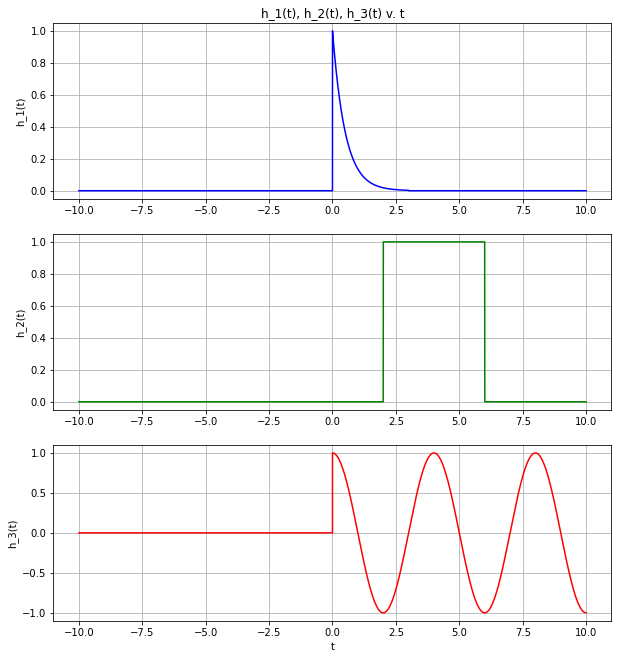
\includegraphics[scale=0.5]{p1t2.png}
  \caption{Part 1, Task 2 - Plots of Python Implementations of \eqref{eq: 1}, \eqref{eq: 2}, \eqref{eq: 3}}
  \label{fig: p1t2}
\end{figure}
\begin{figure}[h!]
  \centering
  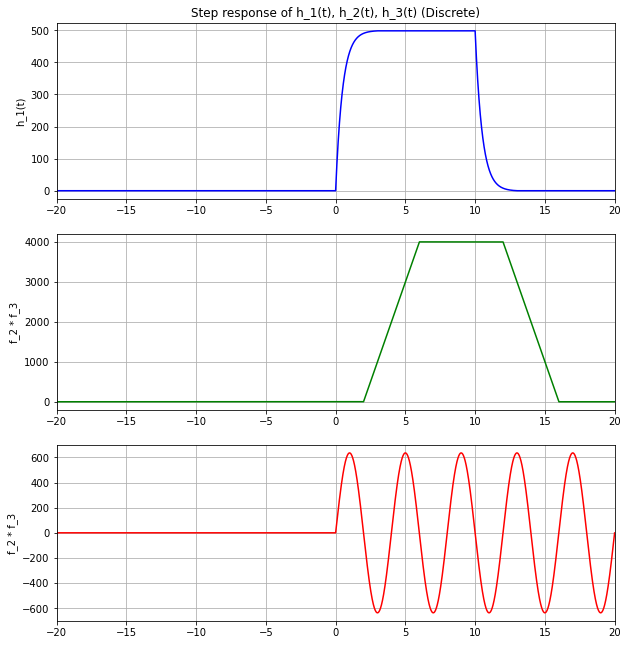
\includegraphics[scale=0.5]{p2t1.png}
  \caption{Part 2, Task 1 - Discrete Step Response of Eq. \eqref{eq: 1}, \eqref{eq: 2}, \eqref{eq: 3}}
  \label{fig: p2t1}
\end{figure}
\begin{figure}[h!]
  \centering
  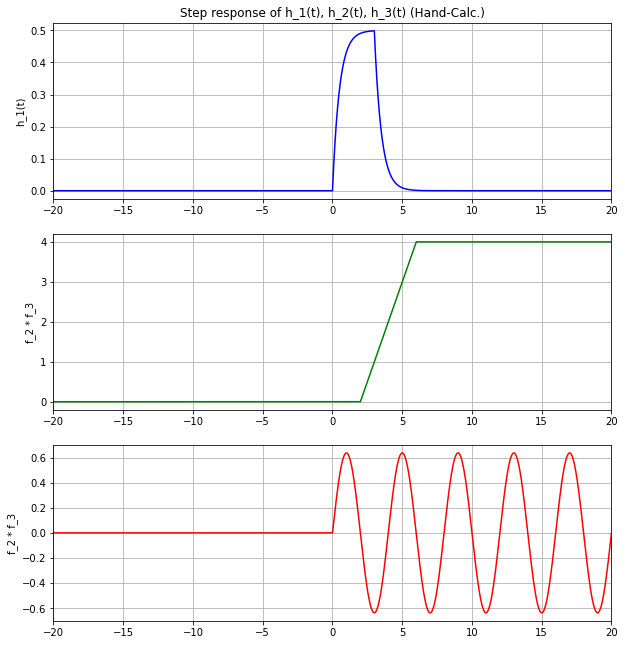
\includegraphics[scale=0.5]{p2t2.png}
  \caption{Part 2, Task 2 - Calculated Step Response of Eq. \eqref{eq: 1}, \eqref{eq: 2}, \eqref{eq: 3}}
  \label{fig: p2t2}
\end{figure}
\section{Error Analysis}\label{section: ErAn}
As can be seen, Figures \ref{fig: p2t1} \& \ref{fig: p2t2} do not look the same. This begs the question, which is correct and why?
Assuming a mistake wasn't made in the hand calculated versions of the step response equations (there wasn't), the reason the sets of plots looks different comes down
to the way the convolution is performed computationally. As the function in \texttt{scipy} used to perform the convolution uses summation, the summation will continue
for the entire length of each function only over the interval given. This is why the plots found computationally can appear stretched or shrunk with respect to the
"true"/calculated step response. 
\section{Questions}
\begin{itemize}
  \item This lab and its tasks were very concise in what is expected for deliverables.
\end{itemize}
\section{Conclusion}
In conclusion, I feel this lab was very successful. The implementation of the code in this lab was quite simple and I really enjoyed seeing the difference in the 
hand calculated and discrete step-response's. This was another useful exercise to show how discrete mathematics can differ from theoretical mathematics. All in all,
I am very satisfied with what this lab has taught me and feel it was an excellent use of time.
\newpage
\thispagestyle{customblank}
\vspace*{\fill}
\centering \section{Attachments}\label{section: Attachments}
\vspace*{\fill}


\includepdf[pages=3, offset=1in -1in]{./attachments/lab4.pdf}

% \begin{thebibliography}{111}
% \thispagestyle{customplain}

% \end{thebibliography}
\end{document}
%This template was created by Roza Aceska.